\chapter{Introduction}

\epigraph{Everything starts somewhere, although many physicists disagree.}{Terry Pratchett, \emph{Hogfather (1996)}}

Despite the fact that quantum mechanics has been established for around a century, only recently have we begun to harness the unique features found in the quantum domain, a development spurred by and further proliferating the rapid progress of experimental advances for quantum systems. It is often control that turns scientific knowledge into technology. Thus control, or the precise manipulation of and interaction with quantum systems, is a fundamental goal of quantum technologies. This may be for the purpose of gaining insight into the physics governing quantum systems, in order to build better devices or in order to solve complex computational problems. We are currently on the cusp of a new age of quantum technologies and control of quantum systems, driven by the methodical exploitation of phenomena such as coherence and entanglement, allowing us to probe and predict the behaviour of quantum systems in ways that could never be done before. 

With this development in experimental capabilities, the demand for theoretical techniques for the time-dependent manipulation of quantum systems has increased considerably. Such techniques are imperative for the development of efficient transformations of quantum states, like in the case of quantum gate design \cite{pelegri_high-fidelity_2022}, quantum computing \cite{albash_adiabatic_2018} or state preparation for the study of condensed matter physics \cite{dimitrova_many-body_2023}, among many other examples. Simultaneously, there has been a rise in demand for techniques which refine and enhance existing protocols with the aim of reducing or mitigating decoherence and unwanted losses, whether through information-theoretic techniques like quantum error-correction \cite{roffe_quantum_2019}, or via approaches for designing driving pulses like in the case of quantum optimal control methods \cite{glaser_training_2015, koch_quantum_2022}. 

\paragraph*{Non-adiabatic losses}

An important example of control imperfections experienced by a system driven in a time-dependent manner is that of losses in the form of undesired transitions that can occur between instantaneous eigenstates of a dynamical Hamiltonian \cite{berry_transitionless_2009, kolodrubetz_geometry_2017}. There are many processes where one might want to end up in \@e.g.~the ground state of a given Hamiltonian whose parameters have been modified in a time-dependent manner. This holds true in the case of state-preparation \cite{dimitrova_many-body_2023}, population transfer \cite{meier_counterdiabatic_2020} or in the case of solutions to combinatorics problems encoded in ground states of Hamiltonians \cite{pichler_quantum_2018, ebadi_quantum_2022}. This is why many quantum driving protocols rely on adiabatic dynamics, where the system follows the instantaneous eigenstates of time-dependent Hamiltonians and transitions are naturally suppressed\cite{born_beweis_1928, kato_adiabatic_1950}. Ideal adiabatic processes are reversible, making them, in principle, highly robust \cite{jarzynski_geometric_1995, kolodrubetz_geometry_2017}. Ideal adiabatic processes, however, require very slow system dynamics and one must make compromises on the timescales of competing heating and decoherence processes. This has led to a rise in the development of methods which aim to speed up adiabatic dynamics while minimising the undesired transitions associated with fast driving, either by entirely removing or by suppressing them. These types of methods are collectively referred to as `shortcuts to adiabaticity' or \acrref{STA} \cite{guery-odelin_shortcuts_2019, torrontegui_chapter_2013}. 

\paragraph*{Shortcuts to adiabaticity} 

The field of \acrref{STA} concerns itself with fast routes to the final results of slow, adiabatic changes of the time-dependent parameters of a system. Such routes are generally designed via a set of analytical and numerical methods for different systems and conditions. Speeding up adiabatic protocols to enable their completion within the system’s coherence time is important
for the development of any quantum technologies relying on such protocols. Thus, \acrref{STA} methods have become instrumental in preparing and driving internal and motional states in atomic, molecular, and solid-state physics. Some \acrref{STA} techniques rely on specific formalisms like invariants and scaling \cite{deffner_classical_2014, deng_superadiabatic_2018, chen_fast_2010}, which exploit symmetries in the physical systems in order to simplify models of non-adiabatic effects, or fast-forward \cite{masuda_fast-forward_2009, masuda_fast-forward_2008}, which adds an external phase to the system wavefunction in order to allow for fast transport. These methods, within specific domains, can be related to each other and potentially be made equivalent because of underlying common structures. A universal \acrref{STA} approach like this is counterdiabatic driving or \acrref{CD}, which will be a focal point of this thesis. 

\paragraph*{Counterdiabatic driving}

The idea of \acrref{CD} was first introduced by Demirplak and Rice in the context of physical chemistry \cite{demirplak_adiabatic_2003} and independently developed by Berry \cite{berry_transitionless_2009}, where it was referred to as `transitionless' driving. The aim of \acrref{CD} is the complete suppression of non-adiabatic effects experienced by a system driven at finite time via the application of an external `counterdiabatic' driving pulse. This is generally not possible, however, due to the fact that the exact counterdiabatic drive is often difficult to compute in the case of complex systems and may be near-impossible to implement in most experimental settings, as well as being undefined for \@e.g.~chaotic systems \cite{kolodrubetz_geometry_2017, pandey_adiabatic_2020, sugiura_adiabatic_2021}. This has led to the development of several approximate \acrref{CD} methods, like the variational approach first introduced by Sels and Polkovnikov in \cite{sels_minimizing_2017} as well as the nested-commutator method of Claeys et al \cite{claeys_floquet-engineering_2019}. Such approaches allow for some suppression of non-adiabatic effects, but their efficacy is highly variable between different systems and the Hamiltonians driving them. Discrete, quantum gate-based versions of \acrref{CD} and its approximations have also been developed, under the moniker of `digitized counterdiabatic quantum optimization' (DCQO) \cite{hegade_digitized_2022}, as well as within the context of the quantum approximate optimisation algorithm or QAOA \cite{wurtz_counterdiabaticity_2022}, although this is a relatively new line of research.

\paragraph*{Quantum optimal control}

A different but complementary approach to achieving the target state of adiabatic dynamics more rapidly is that of quantum optimal control theory or \acrref{QOCT} \cite{glaser_training_2015, koch_quantum_2022}. \acrref{QOCT} is primarily concerned with the development of driving schedules for quantum systems which satisfy specific constraints and behave optimally with respect to a given metric. Links between optimal control and \acrref{STA} have existed throughout the development of both approaches \cite{stefanatos_frictionless_2010, stefanatos_shortcut_2021, zhang_connection_2021}. This has included the realisation of \acrref{CD} through fast oscillations of the Hamiltonian \cite{petiziol_accelerated_2020, petiziol_fast_2018} as well as a fusion of machine learning methods and \acrref{STA}, demonstrating significant improvements for optimizing quantum protocols through machine learning with the inclusion of concepts from \acrref{CD} \cite{bukov_reinforcement_2018, yao_reinforcement_2021, khait_optimal_2022}. While \acrref{QOCT} methods certainly play a part in many aspects of \acrref{STA}, however, they are not applied uniquely to the problem of speeding up adiabatic dynamics. \acrref{QOCT} techniques are often implemented with the goal of driving a system to some desired target state, as in the case of much of \acrref{STA}, however they can also be implemented in determining protocols which satisfy criteria that are unrelated to some target state, like minimising the magnitude of energy expenditure. Due to the versatility of optimal control techniques, they can often be incorporated into many aspects of quantum technologies in order to improve them. Examples include the design of quantum computing gates \cite{pelegri_high-fidelity_2022} as well as improving measurement techniques \cite{wiseman_quantum_2009}, along with the aforementioned applications to speeding up adiabatic dynamics \cite{guery-odelin_shortcuts_2019}.

% Bruno Gavranovic is my love and is good and also is the best and also I love him <3

\paragraph*{Goals and contributions of the thesis}

Speeding up adiabatic processes while suppressing non-adiabatic losses remains an open problem in most practical settings. In the case of \acrref{CD}, issues generally arise at the point of implemention, with the counterdiabatic term requiring operators that are simply not available in an experimental setting, even if the exact counterdiabatic term could be theoretically obtained. The variational approach of Sels and Polkovnikov \cite{sels_minimizing_2017}, which we refer to as `local counterdiabatic driving' or \acrref{LCD}, has attempted to circumvent this by constructing approximations which allow one to choose an ansatz set of operators rather than requiring them to have full support over the exact counterdiabatic drive. Such an approach makes for a far more accessible method, however it is also one which has no guarantees of performance due to the restrictions placed on the operators by \acrref{CD} theory. Optimal control methods, on the other hand, while far more flexible also generally offer very little insight into the way an optimal pulse should be constructed in order to suppress non-adiabatic effects. Thus pure \acrref{QOCT} approaches are often even more ineffective than approximate \acrref{CD} for this purpose. In this thesis, we present a new combination of \acrref{LCD} and optimal control methods which aims to improve upon both of the existing approaches while retaining their advantages. The method, which we will call `counterdiabatic optimised local driving' or \acrref{COLD} \cite{cepaite_counterdiabatic_2023}, is based on the observation that the effectiveness of a given \acrref{LCD} approximation depends on the path of the dynamical Hamiltonian and furthermore, that this path can be optimised using \acrref{QOCT} methods. We will also show that the optimal control component of \acrref{COLD} can be extended by using an optimisation metric constructed using information about the counterdiabatic drive. We will demonstrate the effectiveness and flexibility of \acrref{COLD} and its extensions via numerical analysis, comparing it to both of its components, \acrref{LCD} and quantum optimal control.

\section{Thesis overview}

The thesis is divided into four parts, prefaced by this introduction. \textbf{Part \ref{part:background}} introduces key background concepts relevant to the new results discussed later in the thesis: quantum adiabaticity and quantum optimal control or \acrref{QOCT}. First, we discuss the concept of an adiabatic quantum process, with particular focus in Sec.~\ref{sec:2.1.2_adiabatic_condition} on what it means for a change in the Hamiltonian parameters to be `slow enough' to be adiabatic. We cover how non-adiabatic effects are generated by an operator known as the adiabatic gauge potential (or \acrref{AGP}) and subsequently introduce the concept of a counterdiabatic drive. We then discuss the difficulties of obtaining an exact counterdiabatic drive for a given Hamiltonian and introduce several existing approximations of \acrref{CD}. This includes \acrref{LCD}, which plays a large part in the rest of the thesis. We introduce \acrref{QOCT}, beginning with the mathematical foundations of optimal control as well as several popular numerical optimisation methods. We discuss how optimal control techniques can be applied specifically to quantum systems and describe several \acrref{QOCT} methods that are implemented in order to acquire the results presented later in the thesis.

\begin{figure}[t!]
    \centering
    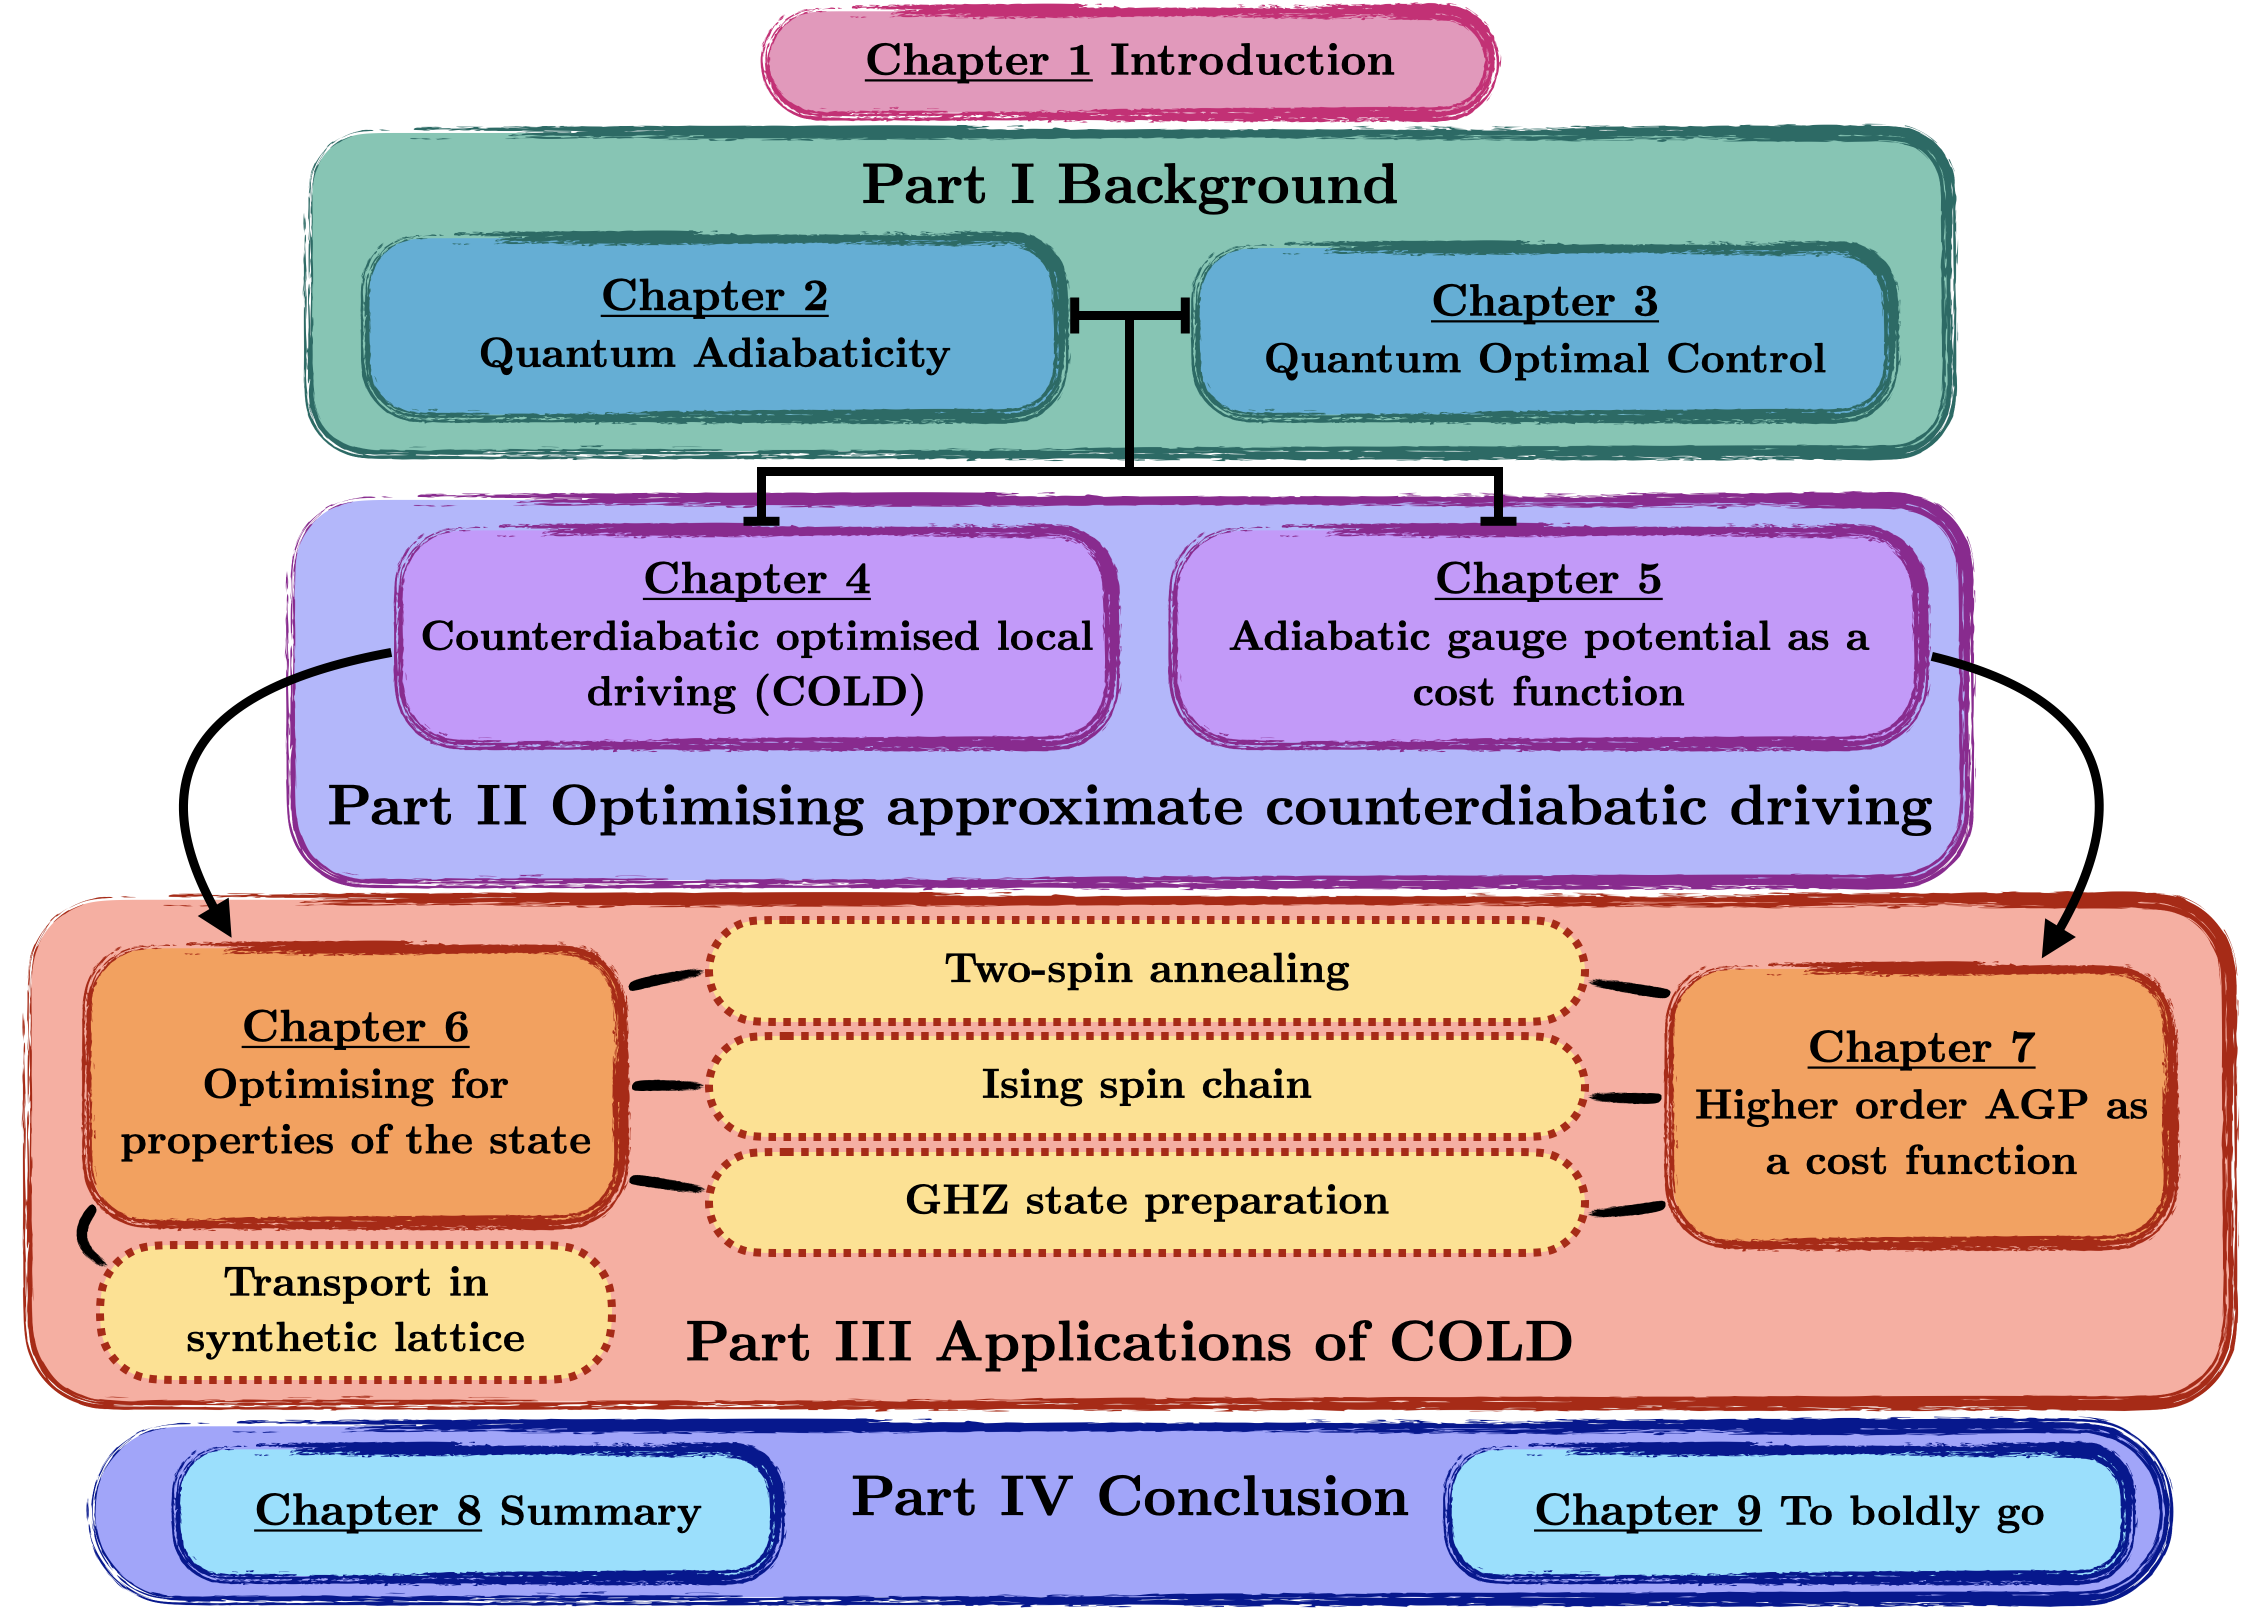
\includegraphics[width=\linewidth]{images/thesis_overview.png} \caption[Thesis outline.]{Thesis outline. In Part~\ref{part:background}, we will introduce the concept of quantum adiabaticity, the counterdiabatic driving (\acrref{CD}) method and its approximations as well as quantum optimal control theory (\acrref{QOCT}) and several optimisation techniques that we will apply later in the thesis. Then, in Part~\ref{part:COLD}, we will combine ideas from \acrref{CD} and \acrref{QOCT} in order to develop a new method for speeding up adiabatic dynamics and the focal point of this thesis: ``Counterdiabatic Optimised Local Driving" or \acrref{COLD}. We will then extend the method with a new optimisation metric based on information about non-adiabatic effects experienced by the system in fast driving. In Part~\ref{part:applications} we will numerically implement the \acrref{COLD} method and its extensions in several different quantum systems to evaluate their performance and compare it to existing techniques. Then, finally, in Part~\ref{part:conclusion}, we will conclude with a summary of the thesis and a look towards the future and several open questions that arise from the work presented here.}\label{fig:thesis_overview}
\end{figure}

In \textbf{Part~\ref{part:COLD}}, we introduce the main new material of the thesis: the \acrref{COLD} method and its extension using several \acrref{AGP}-inspired cost functions. First, we discuss the ways in which \acrref{LCD} and quantum optimal control methods can be combined to obtain better results than either approach alone, and how that follows from the dependence of the counterdiabatic drive on the path of the Hamiltonian in parameter space. We expand on the optimal control methods used for \acrref{COLD} and introduce the idea of using information about the counterdiabatic drive itself, like its total power across the driving time, as a metric for optimising the control pulse in \acrref{COLD} and for the case where no \acrref{LCD} is applied. 

In \textbf{Part.~\ref{part:applications}} we demonstrate implementations of the new methods in numerical simulations of several example quantum systems. First, in Ch.~\ref{chap:6_Applications_fidelity} we present and discuss results obtained when applying \acrref{COLD} to a simple two-spin annealing protocol, the Ising spin chain of varying lengths, the case of population transfer in a synthetic lattice, and finally for the preparation of maximally entangled GHZ states in the setting of frustrated spin systems. We compare the results obtained with \acrref{COLD} to those obtained using un-optimised \acrref{LCD} as well as different optimal control pulses with no counterdiabatic component. In Ch.~\ref{chap:7_higher_order_agp} we do the same but implement \acrref{CD}-inspired cost functions in the optimisation of \acrref{COLD} and plain optimal control instead of using fidelity or (as in the case of GHZ state preparation) entanglement as optimisation metrics. We present results for the two-spin annealing case, the Ising spin chain, and finally for the GHZ state preparation protocol in a system of frustrated spins, to compare and contrast to the case where optimisation is based on final state fidelity. We discuss when such optimisation metrics may be better than those used in Ch.~\ref{chap:6_Applications_fidelity} and in which cases they might fail.

Finally, in \textbf{Part~\ref{part:conclusion}} we conclude with a summary of the thesis and an outlook into future research directions that are left to be explored. A diagram of the thesis structure can be found in Fig.~\ref{fig:thesis_overview}, linking the relevant parts together.

\section{Publications and manuscripts}

The majority of this work is based on the following publications and manuscripts:

\begin{enumerate}
    \item \textbf{Counterdiabatic Optimised Local Driving}, \textit{Ieva Čepaitė, Anatoli Polkovnikov, Andrew J. Daley, Callum W. Duncan. PRX Quantum \textbf{4}, 010309, 2023.} Eprint arxiv:2203.01948. \cite{cepaite_counterdiabatic_2023}
    \item \textbf{Many-body spin rotation by adiabatic passage in
    spin-1/2 XXZ chains of ultracold atoms}, \textit{Ivana Dimitrova, Stuart Flannigan, Yoo Kyung Lee, Hanzhen Lin,  Jesse Amato-Grill, Niklas Jepsen, Ieva Čepaitė, Andrew J. Daley, Wolfgang Ketterle. Quantum Sci. Technol. \textbf{8} 035018, 2023} Eprint arxiv:2301.00218.\cite{dimitrova_many-body_2023}.
    \item \textbf{A numerical approach for calculating exact non-adiabatic terms in quantum dynamics}, \textit{Ewen D. C. Lawrence, Sebastian Schmid, Ieva Čepaitė, Peter Kirton, Callum W. Duncan}, Eprint arxiv: 2401.10985 \cite{lawrence_numerical_2024}.
\end{enumerate}

My contributions to (1) include theoretical work, numerical analysis and writing of the manuscript. In the case of (2) I contributed to some discussions and some numerical analysis relating to the results. In the case of (3), my contribution was confined to theoretical discussions and the writing of the introduction and theoretical component of the manuscript.

\section{Talks and presentations}

Throughout my PhD I gave several talks on my work, including on topics that are not covered in this thesis. Here I list most of them.

\begin{itemize}
    \item \textit{``Solving Partial Differential Equations (PDEs) with Quantum Computers"}, AWE, (March 2020)
    \item \textit{``A Continuous Variable Born Machine"}, \href{https://www.youtube.com/live/ImQeEs0BcQs?feature=share&t=1996}{Pittsburgh Quantum Institute Virtual Poster Session}, Online (April 2020)
    \item \textit{``A Continuous Variable Born Machine"}, \href{https://www.youtube.com/watch?v=6v1IiXRToPU&t=3685s}{Quantum Techniques in Machine Learning}, Online (November 2020)
    \item \textit{``Variational Counterdiabatic Driving"}, University of Strathclyde and University of Waterloo Joint Virtual Research Colloquium on Quantum Technologies, Online (November 2020)
    \item \textit{``A Continuous Variable Born Machine"}, Bristol QIT Online Seminar Series, Online (March 2021)
    \item \textit{``Optimised counderdiabatic driving with additional terms"}, \href{https://meetings.aps.org/Meeting/MAR21/Session/S21.8}{APS March Meeting}, Online (March 2021)
    \item \textit{``Counterdiabatic Optimised Local Driving"}, \href{https://www.youtube.com/watch?v=YkoCPIlFl70}{DAMOP}, Orlando (May 2022)
    \item \textit{``Counterdiabatic Optimised Local Driving"}, QCS Hub Project Forum, Oxford (January 2023)
    \item \textit{``Counterdiabatic Optimised Local Driving"}, \href{https://meetings.aps.org/Meeting/MAR23/Session/Q71.8}{APS March Meeting}, Las Vegas (March 2023)
    \item \textit{``Counterdiabatic Optimised Local Driving"}, \href{https://youtu.be/-btmXDNaQX4}{INQA Seminar}, Online (March 2023)
\end{itemize}